\documentclass[a4paper,11pt]{article}

\usepackage[frenchb]{babel}
\usepackage[utf8]{inputenc}
%\usepackage{verbatim}
\usepackage{graphicx}

\begin{document}
\title{Compte Rendu du TD numéro 4 de l'équipe Eirb'Reteau}
\date{Pour le 7 novembre 2014}
\maketitle

\begin{center}
  Coordinateur : Victor Dury \\
  Tandem 1 : Pierre Gaulon, Reda Boudjeltia \\
  Tandem 2 :  Lionel Adotevi ,  Aurélien Nizet \\
\end{center}
\maketitle
\section{Avant de commencer}
Avant toute chose, il faut remettre les dossiers publique (où Passager et Bus sont des classes abstraites), et factory (où ce sont des interfaces), dans la branche du TD6. Il faut aussi la nouvelle classe PassagerAbstrait, et ainsi certaines modifications sont nécessaires.

\section{Quel lien choisir?}
\subsection{Avec un lien "est-un"}
La première manière de réaliser ces classes est de redéfinir les deux méthodes abstraites, $choixChangerPlace$ et $choixPlaceMontee$.
Voici le diagramme de classe:
\newpage
\begin{figure}[!h]
  \begin{center}
    \caption{Diagramme de classes}
    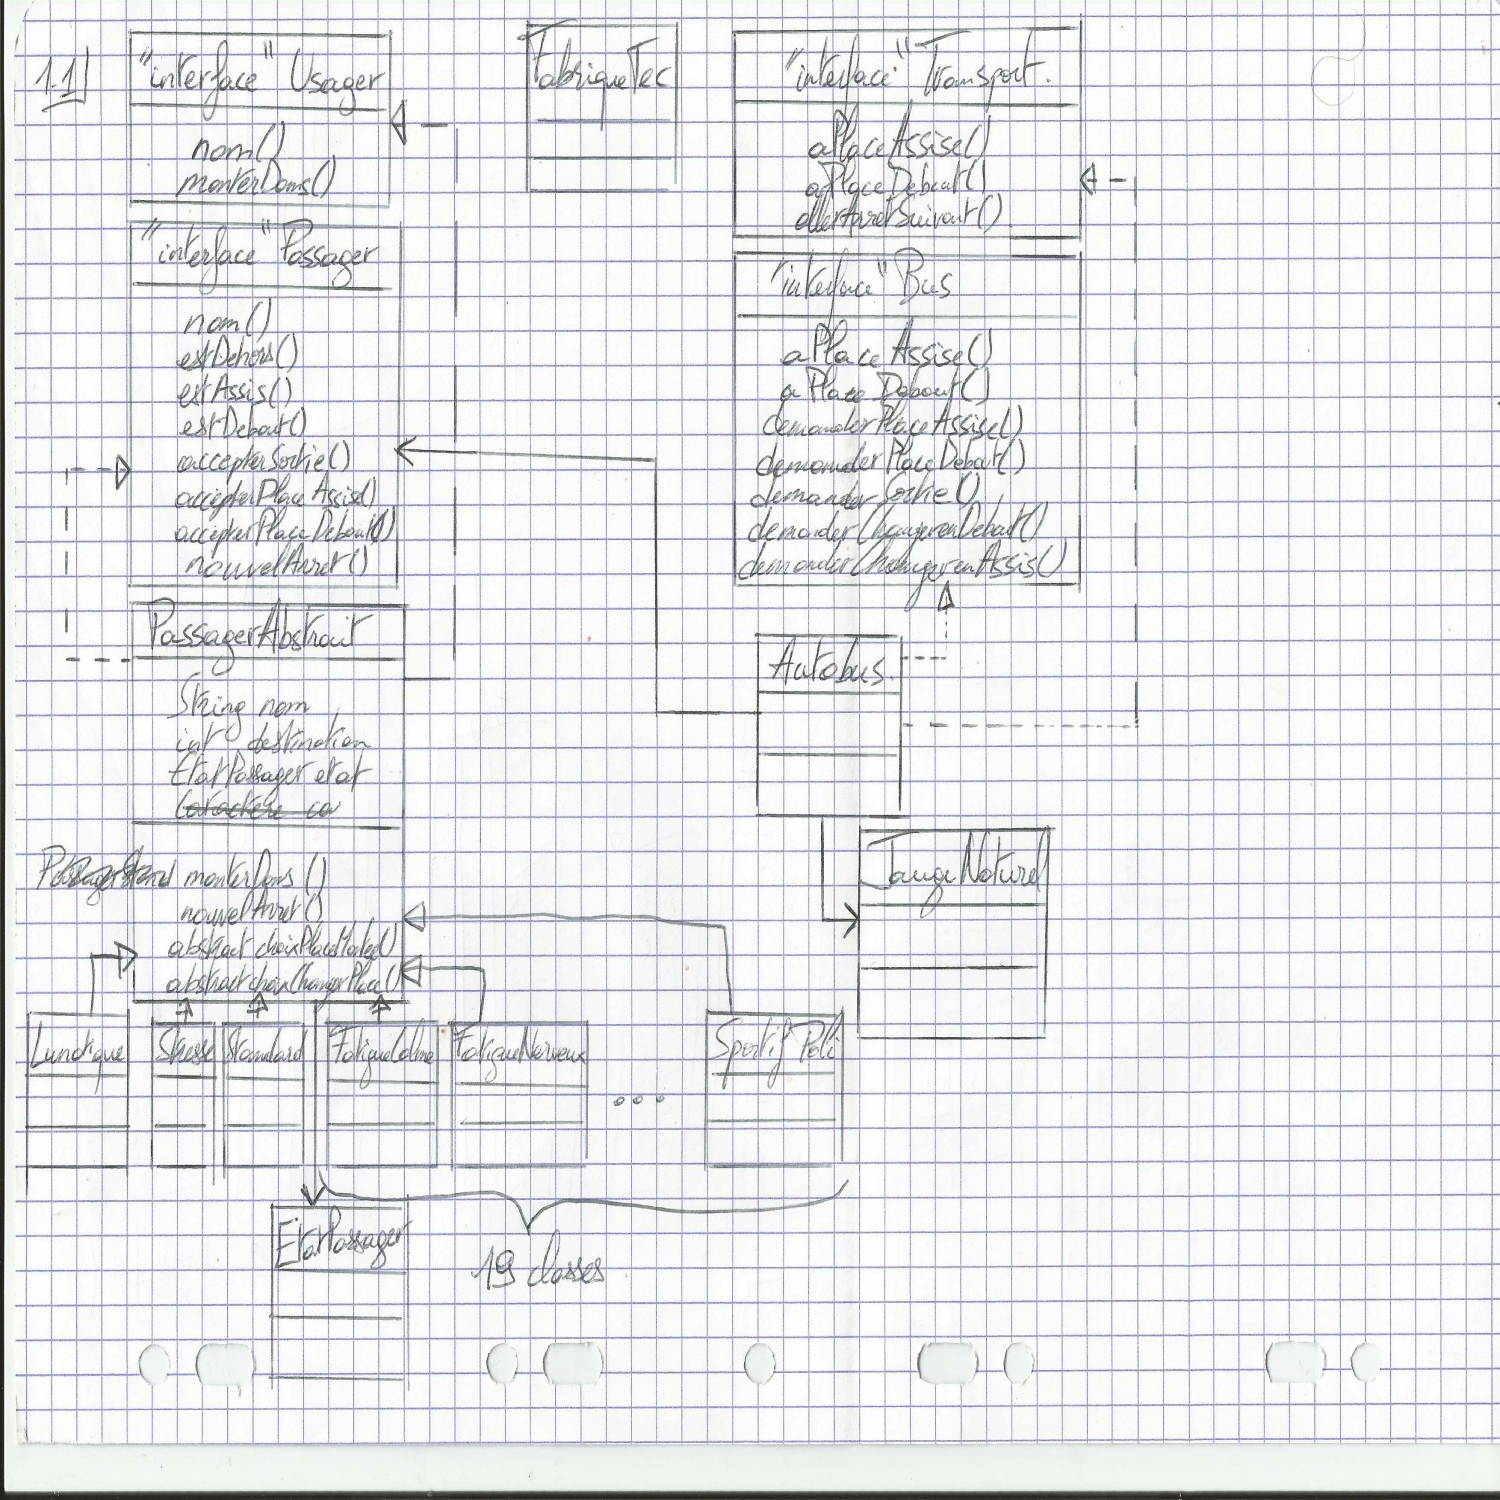
\includegraphics[scale=0.1]{Diag1.jpg}
  \end{center}
\end{figure}
On a ainsi 19 nouvelles classes concrètes, car on doit construire une classe pour chaque combinaison, sachant que la combinaison Repos et Nerveux n'est pas possible. Cette solution n'est donc pas satisfaisante, car on a plusieurs classes contenant le même code. On va donc essayer de le factoriser.

\subsection{Avec un lien "a-un"}
Un lien "a-un" entre deux classes A et B signifie que l'on peut utiliser une instances de A dans la classe B, mais il faut l'instancier avant, et ainsi manipuler une instance différente.
Nous allons donc définir un lien "a-un" entre PassagerAbstrait et les classes caractères Calme, Nerveux, Prudent, Agoraphobe, et Poli, et laisser le lien "est-un" avec les autres.\\
Voici le nouveau diagramme de classe:
\newpage
\begin{figure}[!h]
  \begin{center}
    \caption{FabriqueTec avec caractères "a-un"/"est-un"}
    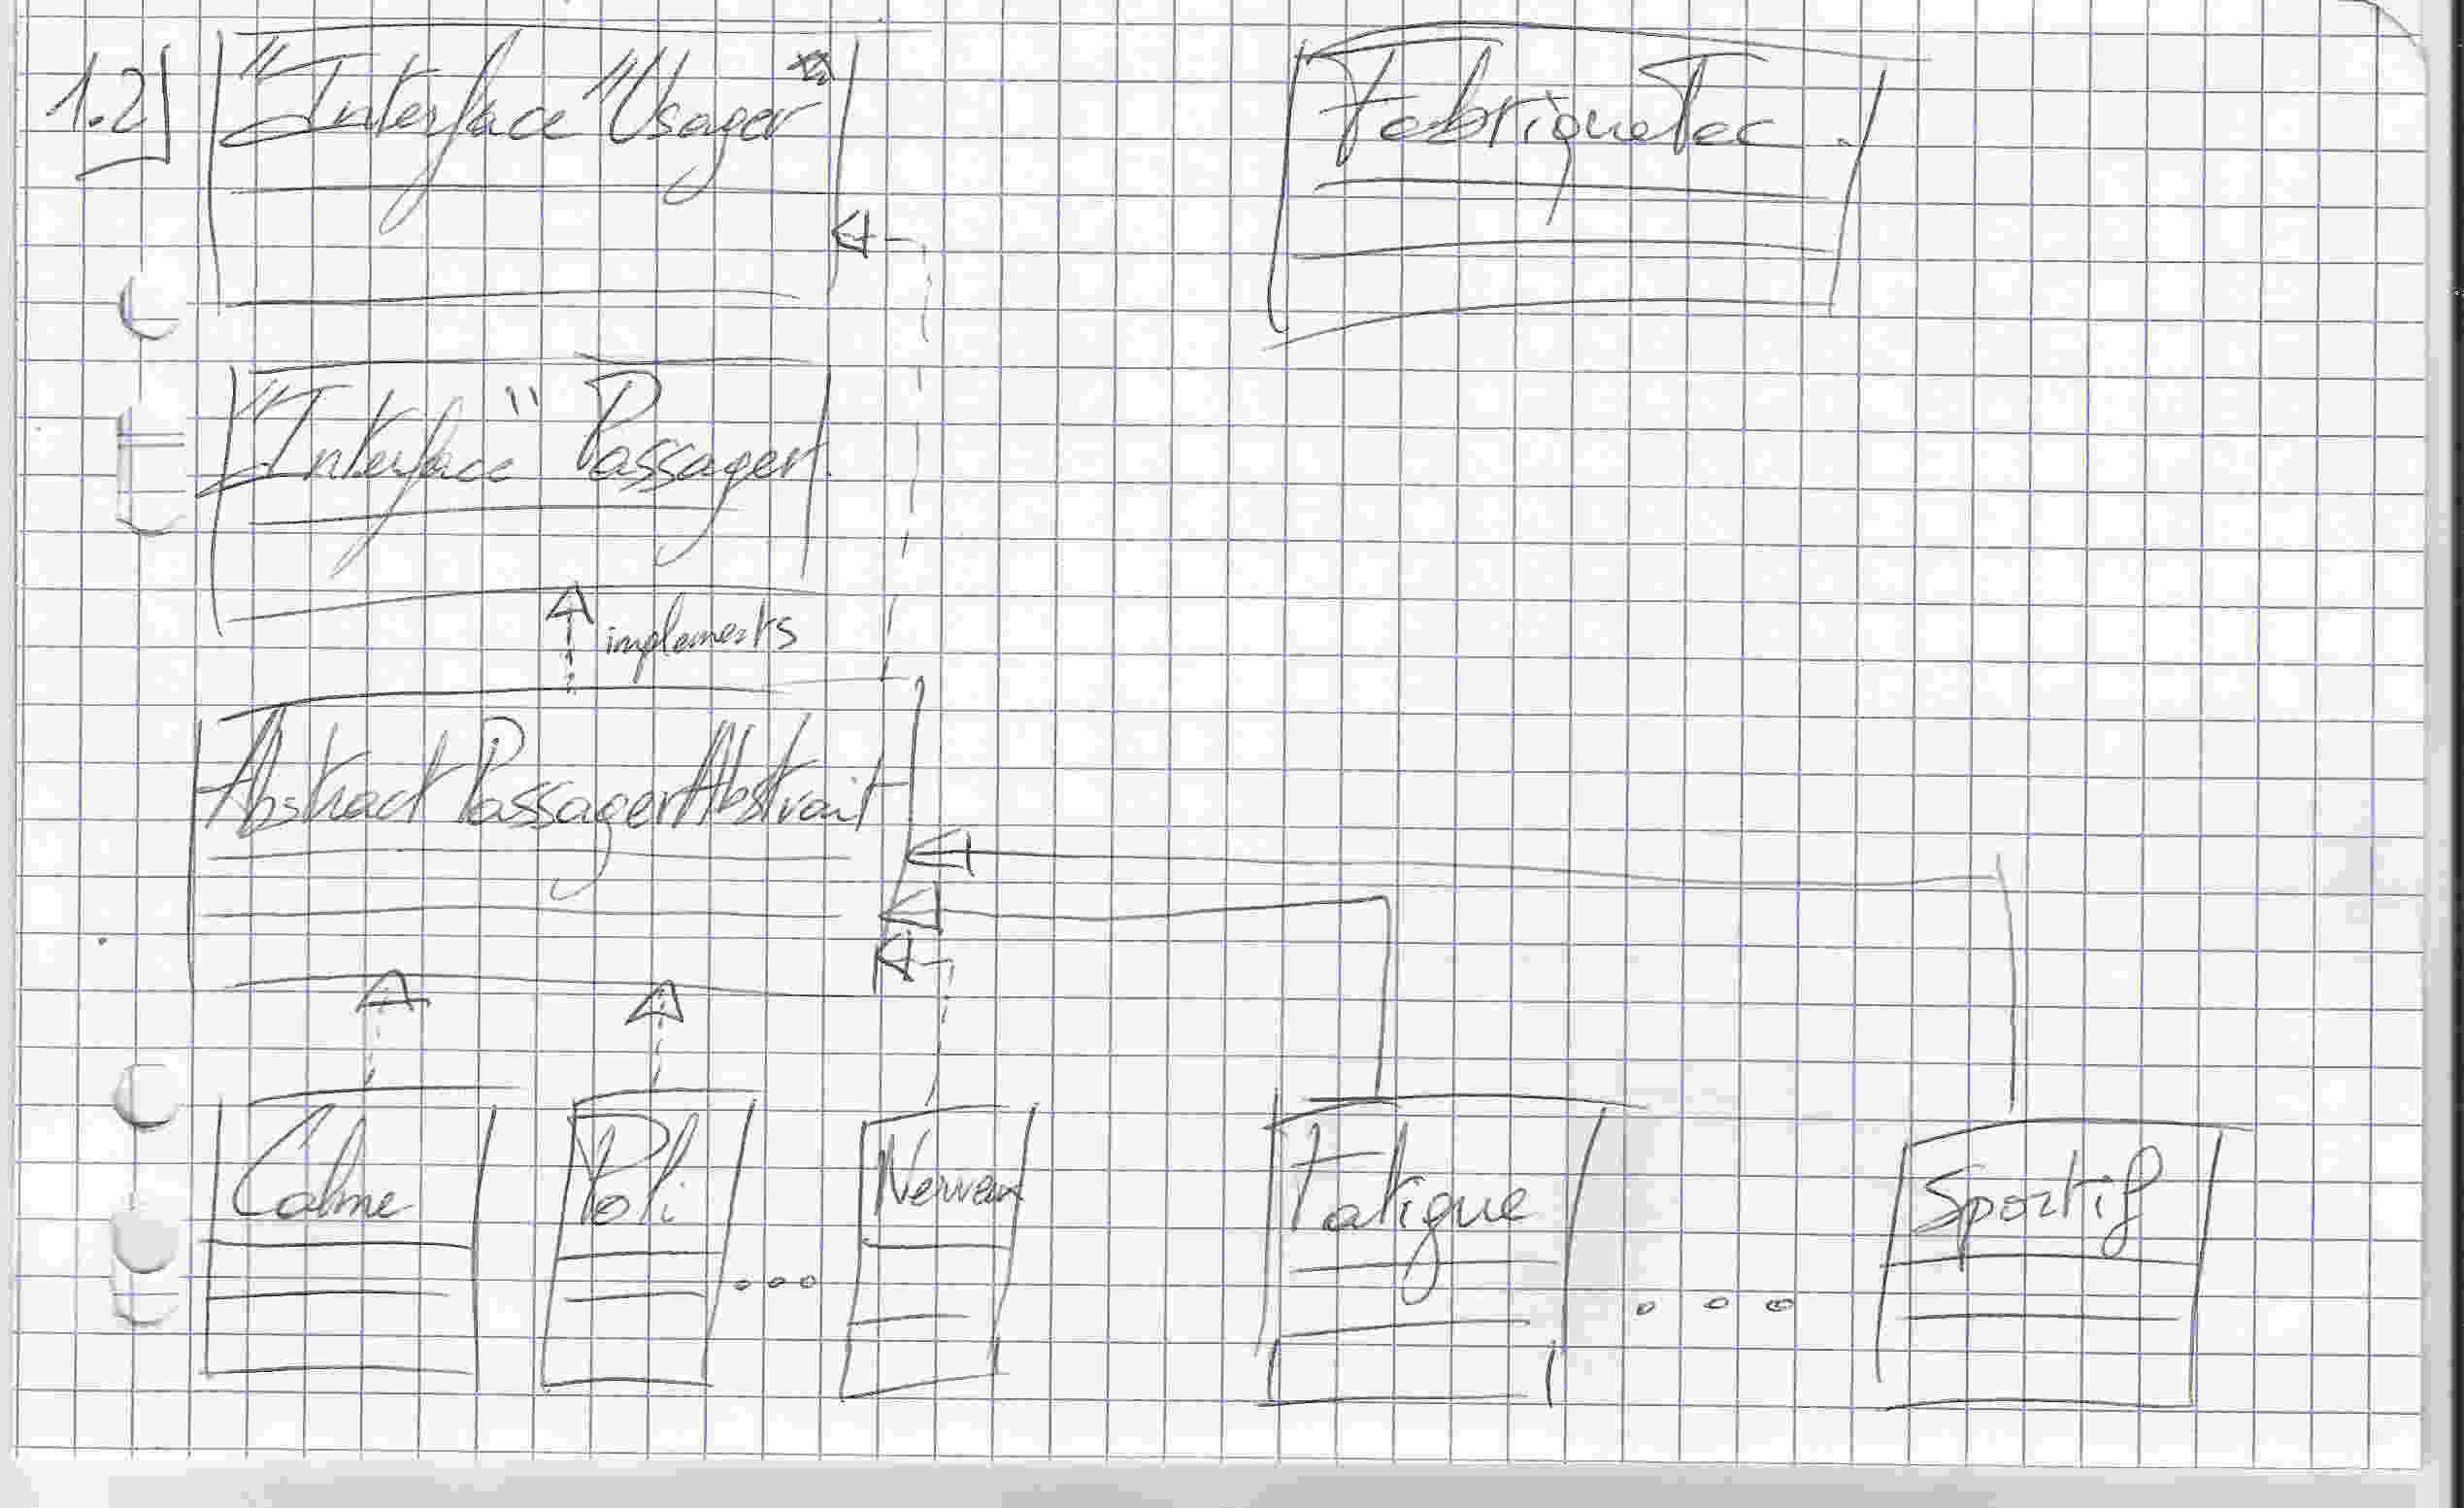
\includegraphics[scale=0.1]{Diag2.jpg}
  \end{center}
\end{figure}

Ainsi, pour la méthode choixChangerPlace(), utilisée par les classes ayant un lien "a-un", on a besoin d'un nouveau paramètre Passager, car ces classes ne sont plus des Passagers. Son nouveau prototype est donc:\\
void choixChangerPlace(Bus b, int arret, Passager p).\\
Si, à la place de mettre le Passager en paramètres, nous le mettons en variable d'instance, il faudrait créer un constructeur par classe pour l'instancier. Avec notre représentation, nos classes ne comportent aucun constructeur et une seule méthode.
\subsection{Boutez vos neurones}
On suppose que java autorise l'héritage multiple.
Ainsi, nous pourrions créer 19 nouvelles classes (toutes les combinaison sauf Repos/Nerveux) à partir des 9 classes créées ci-dessus. Ainsi, nous garderions le même problème que dans la section 1.1. Cependant, nous éviterions la duplication du code.
\section{Réalisation du lien "a-un"}
\subsection{Développement}
Nous avons introduit une interface Caractère, qui définit la méthode choixChangerPlace. Ainsi, elle est implémentée dans les classes Calme, Nerveux, Prudent, Agoraphobe, et Poli. Ensuite, on appelle ces caractères dans les contructeurs des classes Sportif, Poli, Fatigue, et Tetu.\\
Par contre, dans fabrique, on instancie les caractères dans FabriqueTec, alors que dans publique, on les instancie dans les constructeurs. 
Les représentations de la fabrique et de publique sont les mêmes au niveau des diagrammes de classes, à part Passager et Bus qui peuvent être une interface ou une classe abstraite. 
Voici le diagramme de classes de ces représentations:

\begin{figure}[t]
  \begin{center}
    \caption{FabriqueTec avec Caractère}
    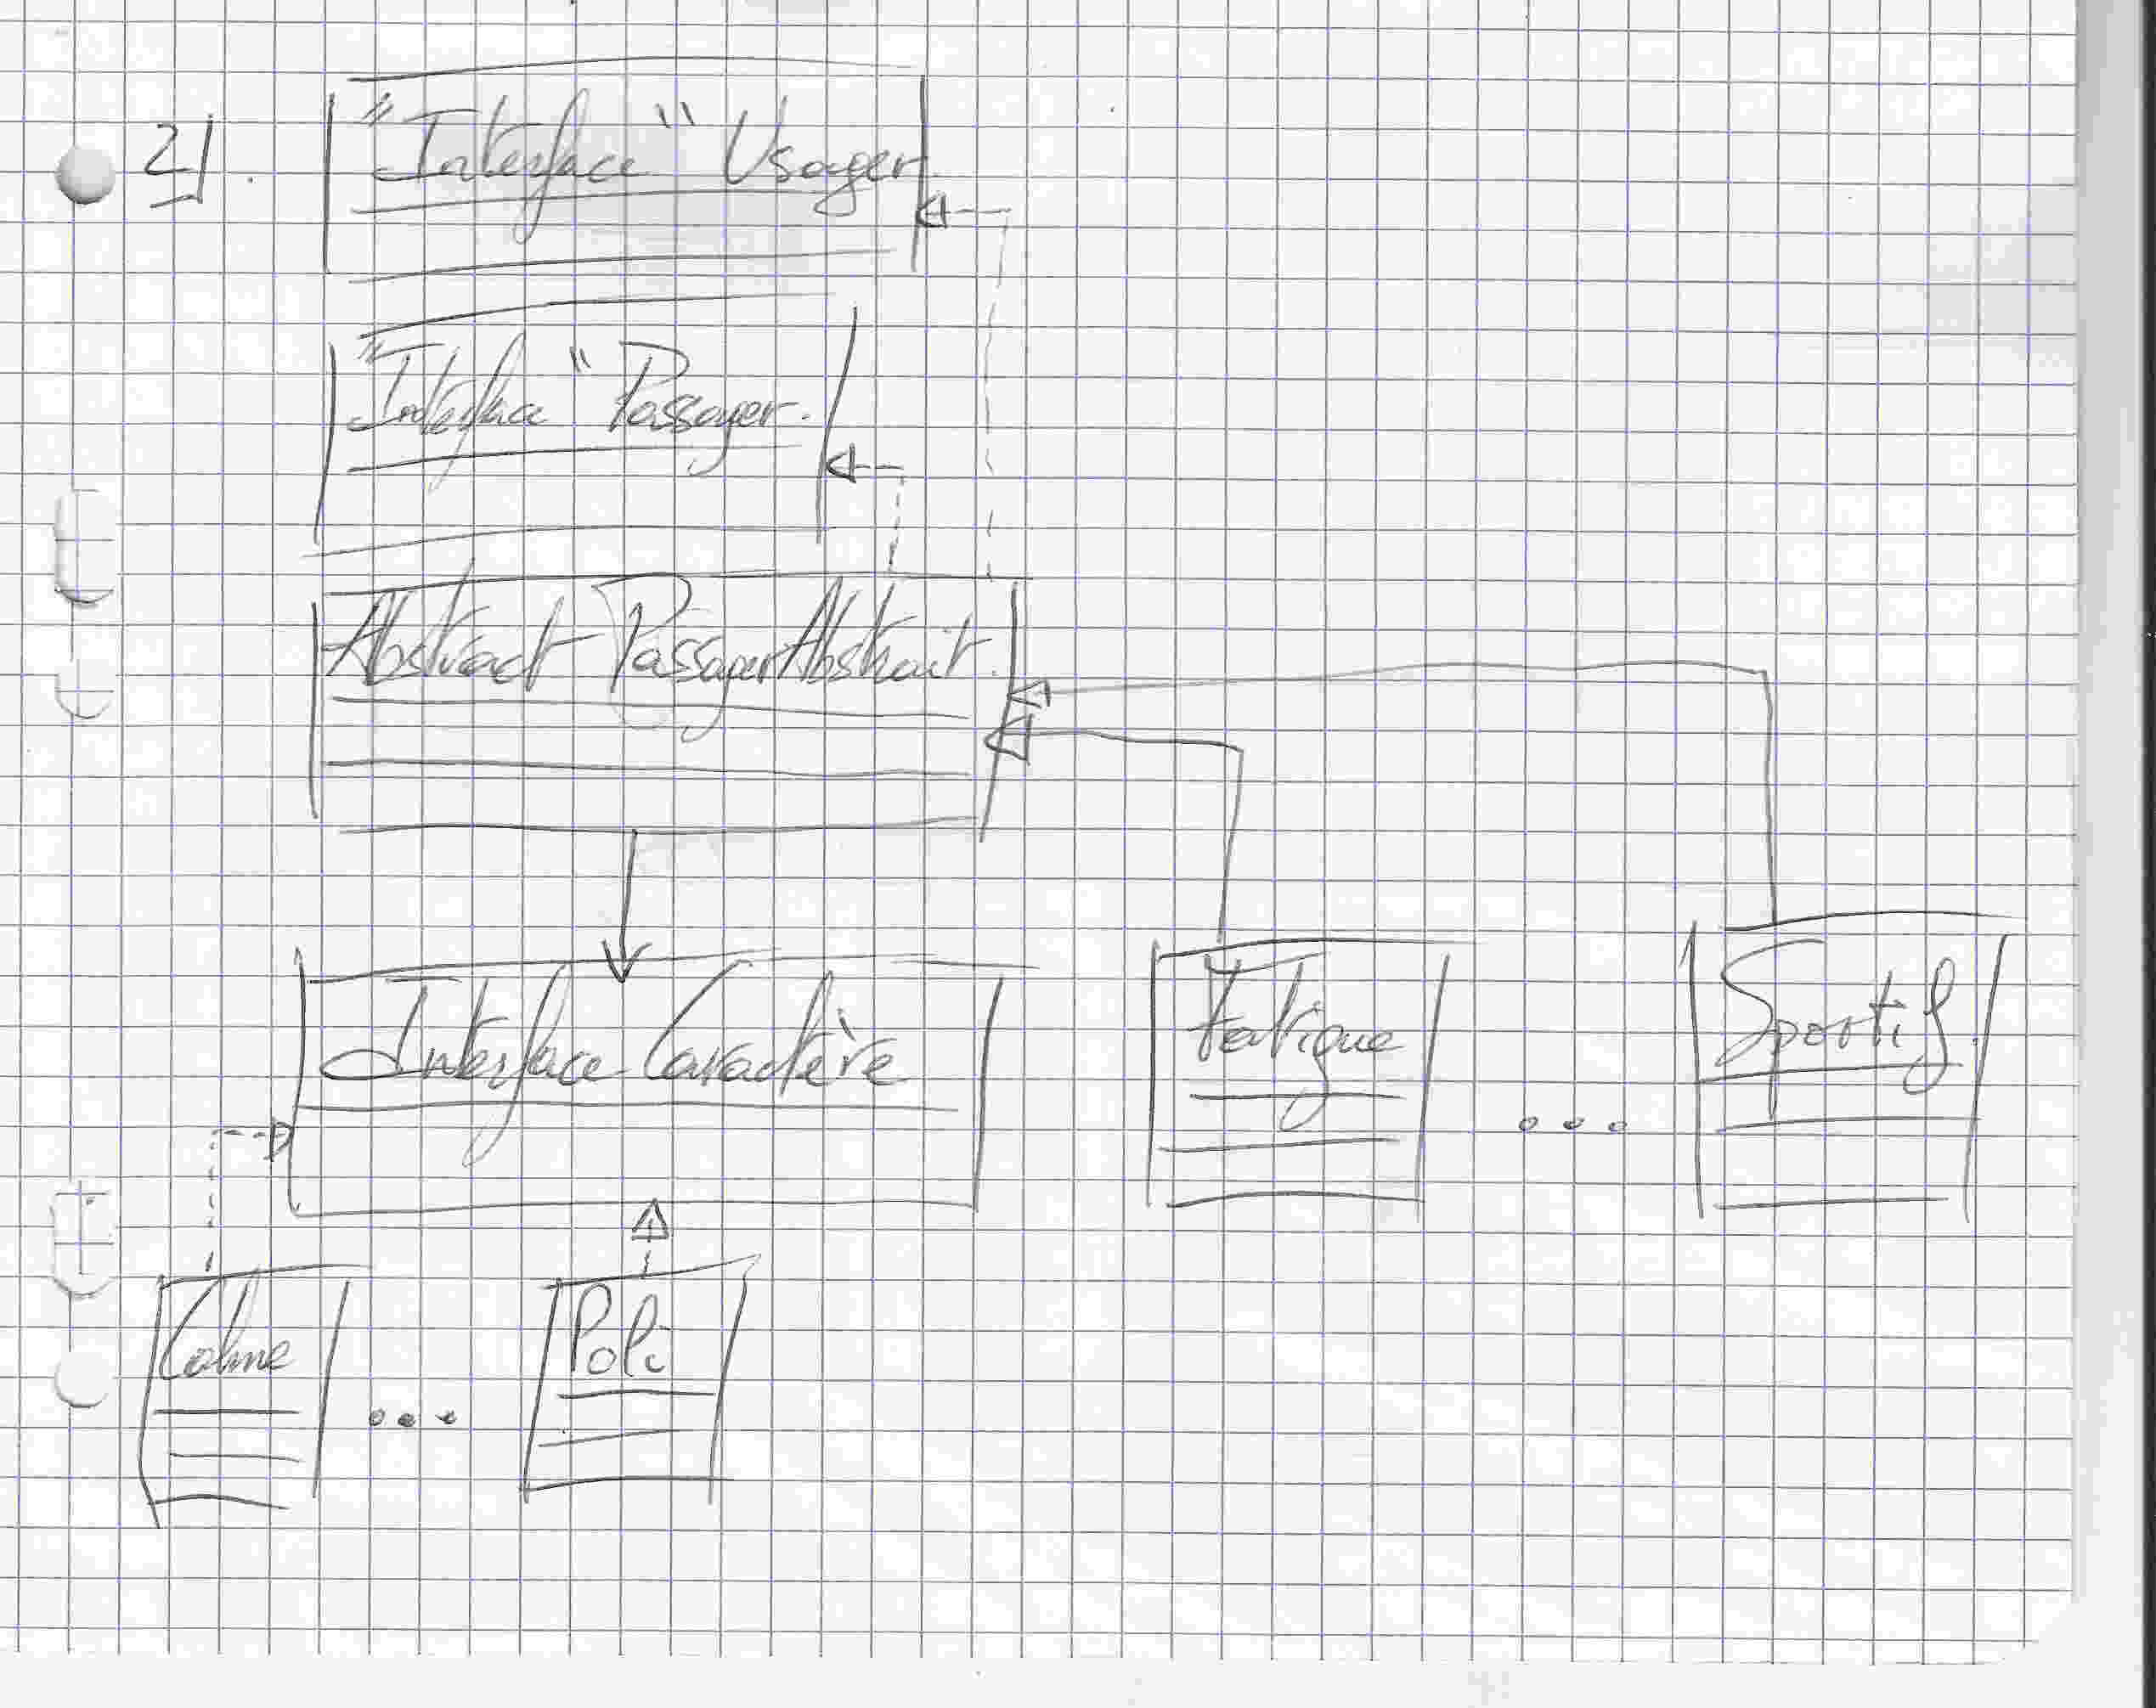
\includegraphics[scale=0.1]{Diag3.jpg}
  \end{center}
\end{figure}

\subsection{Boutez vos neurones}

Dans la première solution, on peut instancier les caractères autant que l'on veut, notamment dans d'autres classes, alors qu'avec le singleton, on ne pourra l'instancier qu'une seule fois, et dans la classe concernée.

\section{Commentaires}

\begin{itemize}
\item Pierre: J'ai trouvé que le fait de revenir à une architecture avec deux branches a été plus perturbant que bénéfique. La difficulté a été de se répartir les différentes tâches tout en tenant compte des différences des deux solutions. Et le développement des tests, de la même manière en tenant compte des différences des deux branches a été plus long que le développement en lui même. Je pense qu'on espère qu'on va gagner.
\item Victor: Ce projet nous a permis de comprendre que l'on peut implémenter un désir fonctionnel grâce à plusieurs solutions techniques. Encore une fois, ce TP nous a permis de se questionner sur l'heritage multiples, ses possibilités, et contraintes. Moi personnellement, en tant que coordinateur, ce projet m'a permis de réaliser la condition nécessaire à la prise de décision dans l'intérêt général.
\item Aurelien :  Lors de ce TD nous avons pû remettre en question les différentes solutions de réalisation à l'instar des contraintes fonctionnelles modelisant le comportement des différentes méthodes. En outre, en considérant l'ensemble des différents problemes analysés séparément et non dans un contexte communs, nous sommes parvenus à des conclusions hâtives. Qui plus est l'héritage multiple permet de répondre à ces contraintes dans une moindre mesure qui n'est pas adapté au langage.
\item Lionel: La création des instances de Passagers menant à un aboutissement personnel, que j'ai quelque part souhaité, m'a mené à cette réflexion. Dès lors, chaque individu étant présupposé rationnel, et poursuivant en priorité son propre intérêt, il en ressort que les hommes souhaitent naturellement sortir de cet état de nature mortifère, où personne ne peut gagner. Le bus est une façon pour les passagers de s'extraire de leur condition et de s'instancier dans le monde de la conscience propre, ce qui fait d'eux des objets à part entière.
\item Reda : Celui qui, se trouvant déjà lié par quelque union originelle de paquetages, d'intérêt ou de convention, n'a point encore porté le vrai joug des lois. Celui qui n'a ni méthodes, ni attributs bien qu'encapsulé; celui qui ne craint pas d'être accablé par un accès mal intentionné; qui, sans entrer dans les classes de ses voisins, peut résister seul à chacun d'eux, ou s'aider de l'un afin de s'assoir dans le bus.

\end{itemize}


\end{document}
